\chapter{红外无人机目标检测相关理论}

\section{人工神经网络}
人工神经网络又称为类神经网络,一般简称神经网络。在机器学习领域中是一种模仿生物的神经网络结构的计算模型。这种模型常常被用来估计一种未知的函数。神经网络由大量的人工神经元组成,并能借助外界的信息改变内部结构,也就是具备学习功能。在很多领域,神经网络能有类似人类的决定能力,因此很多传统编程方法难以解决的问题都可以用神经网络来进行解决。

典型的人工神经网络具有以下三个部分:

(1)结构:结构指定了网络中的变量和它们的拓扑关系。例如,神经网络中的变量可以是神经元连接的权重和神经元的激励值。

(2)激活函数:部分神经网络模型具有一个短时间尺度的动力学规则,来定义神经元如何根据其他神经元的活动来改变自己的激励值。一般激励函数依赖于网络中的权重(即该网络的参数)。

(3)学习规则:学习规则指定网络中的权重如何随时间调整。 这通常被认为是一个长期的动力学规则。 一般来说,学习规则取决于神经元的激发值。 它也可能取决于主管提供的目标和当前权重值。 例如,用于手写识别的神经网络有一组输入神经元。 输入神经元由来自输入图像的数据激发。 激励值经过加权并通过一个函数(由网络设计者确定)后,将这些神经元的激励值传递给其他神经元。 这个过程一直重复,直到输出神经元触发。 最后,输出神经元的激发值决定了识别的字符。

\section{卷积神经网络}
卷积神经网络区别于其他神经网络模型,比如递归神经网络、玻尔兹曼机等,
它最大的不同在于卷积操作,使卷积神经网络在目标检测、图像分类、自然语言
处理等计算机视觉任务上效果显著。卷积神经网络的主要结构如图\ref{cnn}所示,
由输入层、卷积层、激活函数、池化层、全连接层和输出层组成。对于目标检测
所使用的卷积神经网络还会包含目标函数、非极大值抑制等。下面介绍卷积神经
网络的各个部分的结构。

\begin{figure}[htbp]
    \centering
    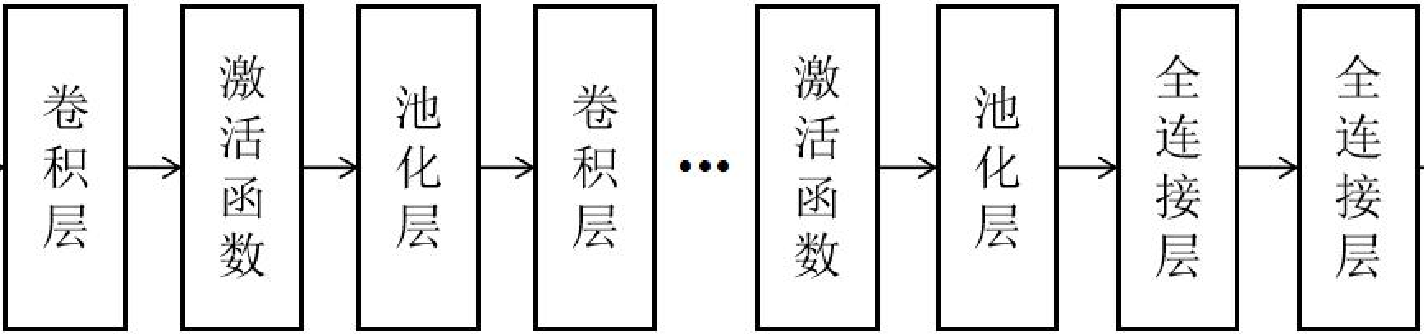
\includegraphics[width = 0.9\textwidth]{cnn.png}
    \caption{卷积神经网络常见结构}
    \label{cnn}
\end{figure}

\subsection{卷积层}
卷积层是卷积神经网络的重要组成部分之一,卷积运算实际上就是分析数学
中的一种运算方式,在卷积神经网络中最主要用到的是离散卷积运算。卷积运算的公式可以写作如式\ref{conv1}所示:
\begin{equation}
    \mathrm{s}(t)=\left(x^{*} w\right)(t)
    \label{conv1}
\end{equation}

\begin{figure}[htbp]
    \centering
    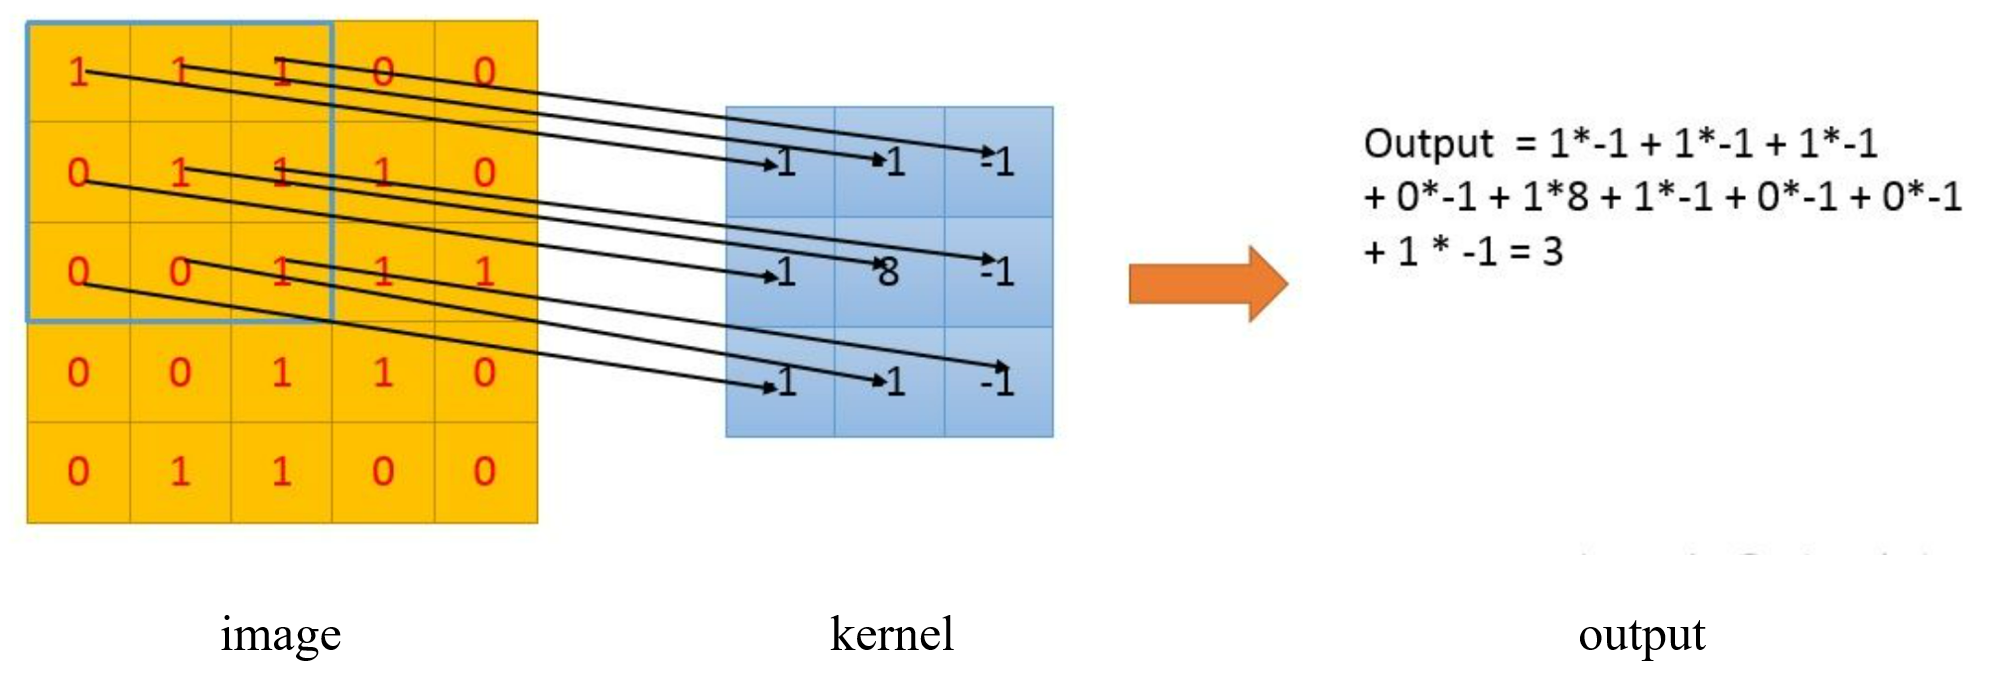
\includegraphics[width = 0.9\textwidth]{jjgc.png}
    \caption{图像卷积运算过程}
    \label{jjgc}
\end{figure}

其中$x$代表输入,$w$ 代表核函数。应用在图片上的卷积可以看做是二维矩阵
的乘法,卷积核的大小要远小于图像的大小,因此卷积可以看做是一种局部操作。
对图像的卷积过程如图\ref{jjgc}所示,
假设输入图像为$5\times5$的矩阵,卷积核的大小为
$3\times3$,卷积操作从图像左上角开始,即$(0,0)$坐标,本次卷积后的结果为卷积
核中的数值与图像对应位置的像素值逐位相乘后累加,之后卷积核以设定的步长
为移动单位从上到下从左到右的在图像上依次进行卷积,最终输出结果(在目标
检测中也称为特征图),结果的大小由式\ref{cout}决定,
\begin{equation}
    N_{\text {output }}=\frac{\left(W_{\text {input }}-F+2 P\right)}{S}+1
    \label{cout}
\end{equation}

其中$W$代表输入图像大小,$F$ 代表卷积核大小, $P$ 代表 padding 的像素数,$S$ 代表步长。卷积核参数的不同
即代表了不同的特征提取能力,通过不同的卷积核作用于图像获得图像不同的局
部信息,比如边缘、纹理、形状等。卷积神经网络实际上就是不同的卷积核进行
组合,浅层的卷积主要提取图像的细节信息,深层的卷积则主要获得语义信息,
在网络进行误差反向传播时更新卷积核的参数来增强网络的学习能力。

\subsection{激活函数}
激活函数的引用是为了解决网络的非线性问题,增加整个网络的表达能力,
激活函数的初衷是模拟了生物神经元特性,解决之前简单线性加权难以解决的非
线性信号拟合问题。常用的激活函数如下:

(1)Sigmoid 函数:也称 Logistic 函数,该函数的数学定义式为\ref{log}所示,
\begin{equation}
    \sigma(x)=\frac{1}{\exp (-x)+1}
    \label{log}
\end{equation}

\begin{figure}[htbp]
    \centering
    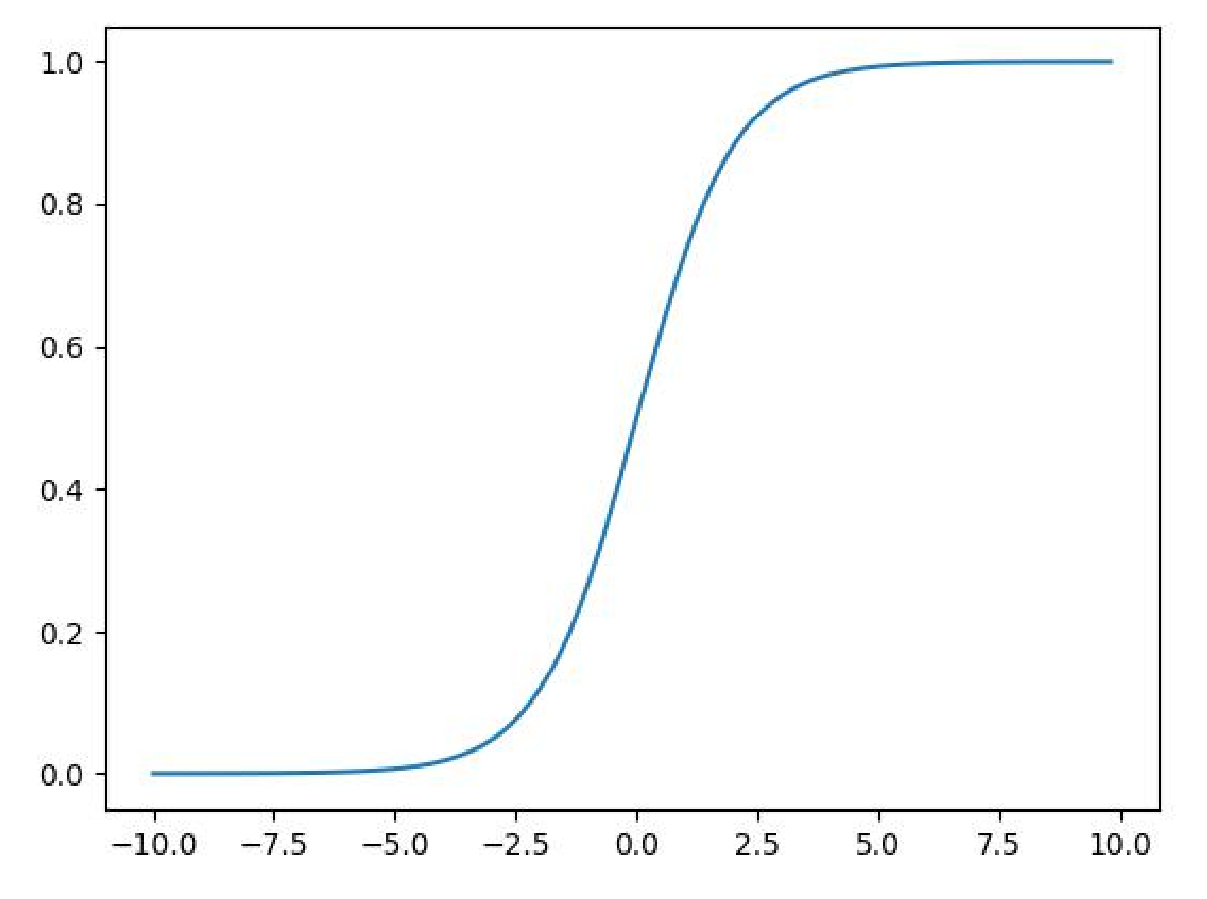
\includegraphics[width = 0.5\textwidth]{sigmoid.png}
    \caption{Sigmoid函数}
    \label{sig}
\end{figure}

\begin{figure}[htbp]
    \centering
    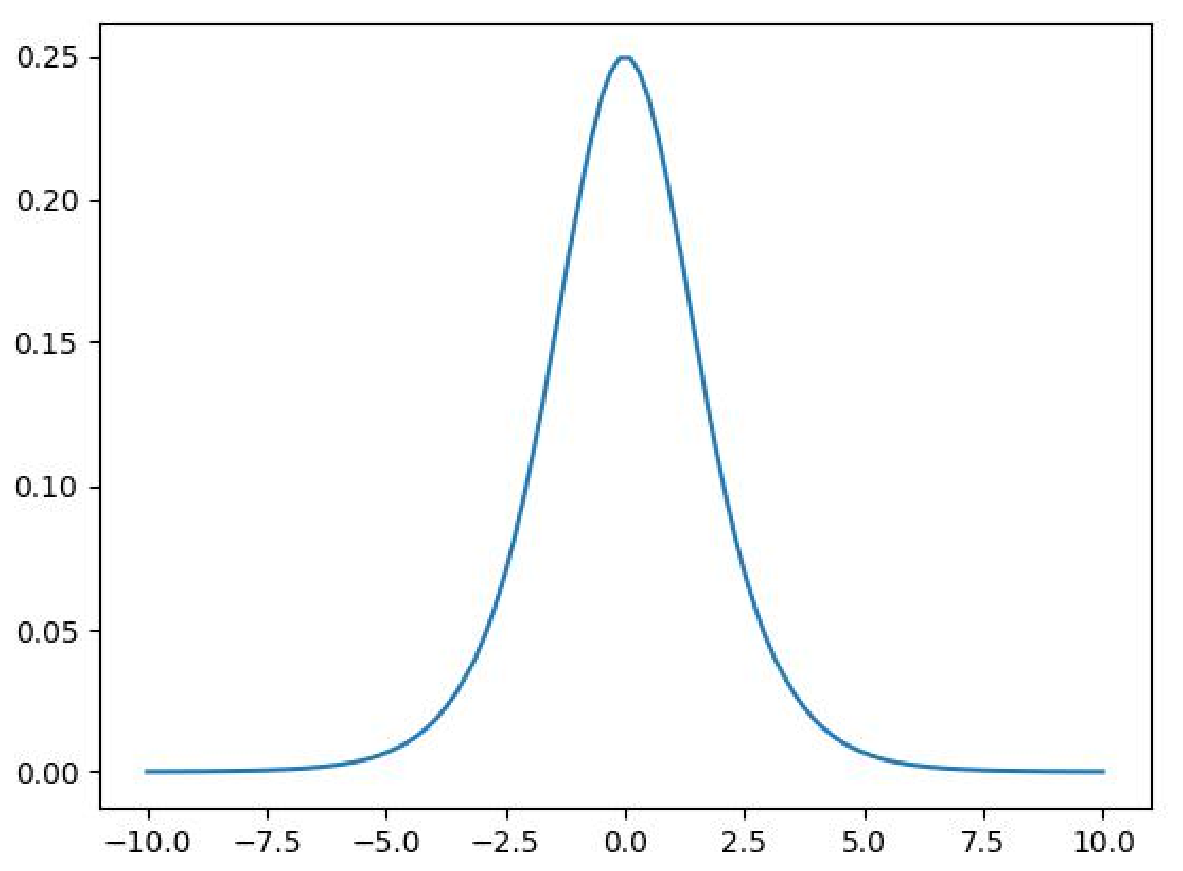
\includegraphics[width = 0.5\textwidth]{sig导数.png}
    \caption{Sigmoid导函数}
    \label{sigd}
\end{figure}

其函数图像如图\ref{sig}所示,从函数图像可以直观的看出经过 Sigmoid 函数处理后
将输出范围压缩到$[0,1]$之间,可以用于二分类,从其导数图\ref{sigd}可以看出
Sigmoid 函数易于求导,但其存在最大的局限就是当输入较大或较小时进行误差
反向传播时会出现“梯度消失”的情况,导致网络训练无法正常训练。为了避免
出现梯度消失的情况出现,后面又提出了 ReLU 函数作为替代。

(2)Tanh 函数:又叫做双曲正切激活函数,该函数是为了解决 Sigmoid 函
数均值问题提出的。该函数的数学定义式为\ref{tanh}所示,
其函数图像如图\ref{tanh}所示,
从函数图像可以直观的看出经过 Tanh 函数处理后的输入输出范围压缩到$[-1,1]$
之间,并且图像是以原点为中心旋转对称的,可以将 Tanh 函数看做是 Sigmoid
函数进行拉伸和下移得来的,解决了 Sigmoid 函数的 zero-centered 问题,避免随
着网络深度的加深,后一个神经元的输出不断影响下一层神经元导致数据分布改
变的问题。在实践中 Tanh 函数比 Sigmoid 函数效果更好,但仍然没有解决梯度
消失的问题。
\begin{equation}
    \sigma(x)=\tanh (x)=\frac{\exp (x)-\exp (-x)}{\exp (x)+\exp (-x)}=2 \operatorname{sigmoid}(2 x)-1
    \label{tan}
\end{equation}

\begin{figure}[htbp]
    \centering
    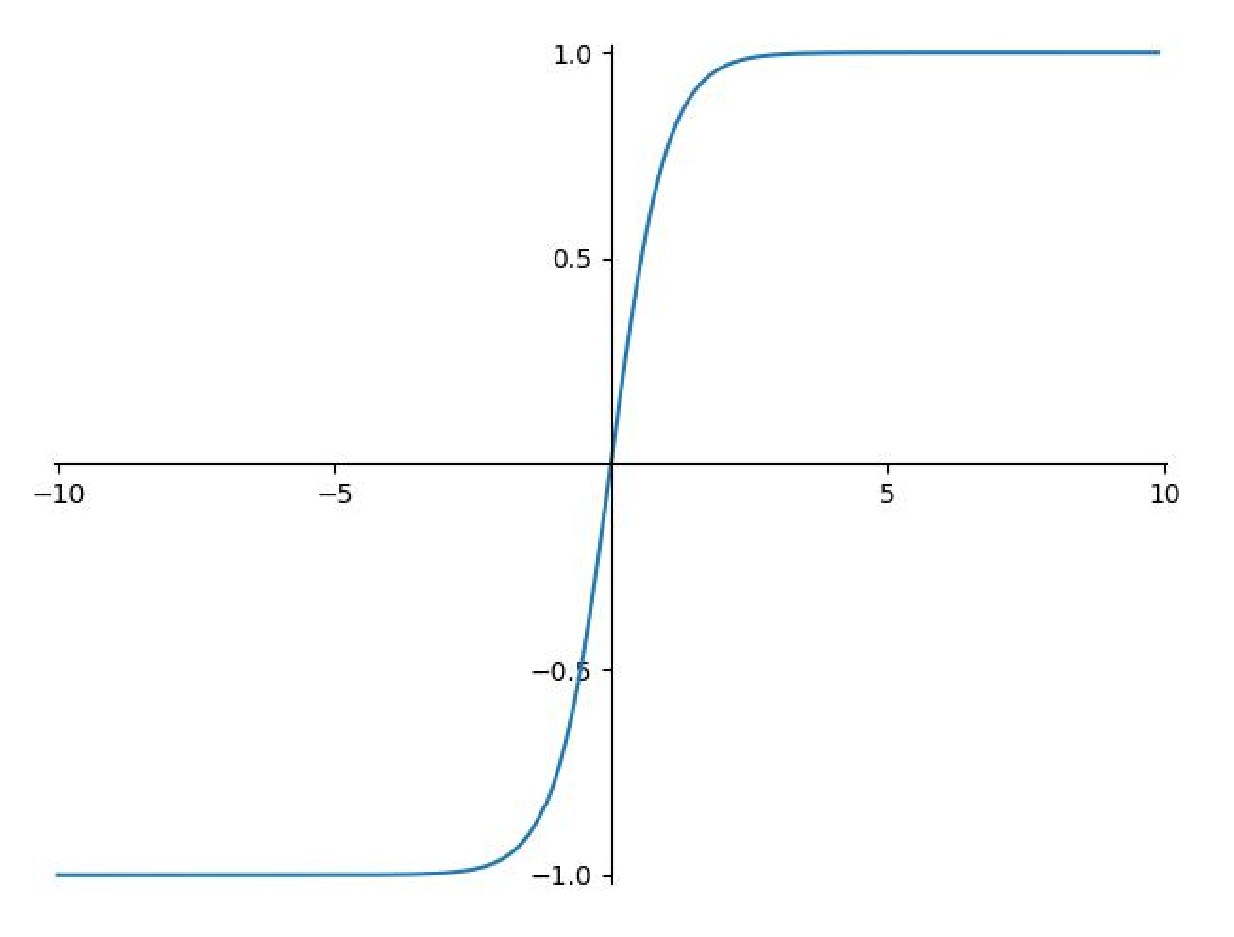
\includegraphics[width = 0.5\textwidth]{tanh.png}
    \caption{Tanh函数}
    \label{tanh}
\end{figure}

(3)ReLU 函数:该函数的数学定义式为式\ref{relu}所示,该函数是在 2010 年
Hinton 和 Nair 提出,可以看出 ReLU 在$x\ge 0$时导数为 $1$,有效地解决了梯度消
失问题,是目前神经网络中最常用的激活函数之一\cite{xu2015empirical}。ReLU 函数相对于前两个
激活函数公式非常简单,是一个分段函数,在计算速度上也非常快,在实践中发
现 ReLU 函数收敛速度也比 tanh 函数快 6 倍以上。但 ReLU 强行将$ x<0$的部分
置于 0,会导致这部分神经元处于“死区”,因此不能将学习率设置的过大。后
续研究者针对以上的问题提出了 LeakyReLU\cite{maas2013rectifier}、PReLU、RReLU 等变体。
\begin{equation}
    \sigma(x)=\max (0, x)= \begin{cases}x & x \geq 0 \\ 0 & x<0\end{cases}
    \label{relu}
\end{equation}

\subsection{池化层}
卷积神经网络中一个典型组件包括三个部分:第一部分,并行计算多个卷积
产生线性特征输出。第二部分,通过激活函数对上一级输出增加非线性关系。最
后一个部分,通过池化函数调整输出特征大小。池化层也叫下采样层,主要通过
池化函数进行“降采样”,池化函数的计算过程为某一位置的输出代表着原位置
邻域的总体特征,过程如图\ref{maxp}所示。常用的池化函数主要有最大值池化函数
(Max-pooling)、平均值池化函数(Average-pooling)、基于像素距离的加权平均
函数等。池化层的主要功能有:

(1)特征不变形。以最大值池化为例,其池化
操作是对某一位置附近的最大值比较敏感,而不是具体的位置,因此能够容忍特
征的少量位移。

(2)特征降维。由于池化操作就是进行“降采样”,池化后结
果的每一个位置都对应原特征图的一个子区域,因此池化操作就相当于对特征图
进行空间上的压缩。

(3)经过池化层后的输出减小,输入下一层后自然就降低
了计算量和参数,因此在一定程度上能够防止过拟合\cite{gu2018recent}。

\begin{figure}[htbp]
    \centering
    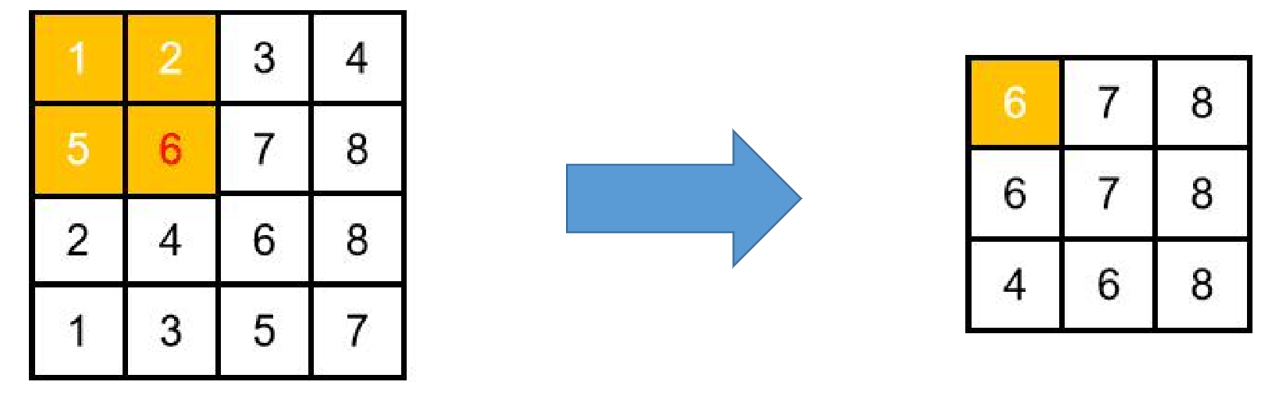
\includegraphics[width = 0.9\textwidth]{maxp.png}
    \caption{最大池化示意图}
    \label{maxp}
\end{figure}

\subsection{全连接层}
全连接层处于卷积神经网络最后几层,用于将卷积层、池化层和激活函数等
操作获得到的特征进行综合起来,起到“分类器”的作用。由于全连接层要求特
征向量输入大小固定,因此目前主流的目标检测网络都选择用卷积层来代替全连
接层,起到提高检测速度的目的。

\section{目标检测的评价指标}
目标检测结果的优劣主要由两个指标来评价:(1)平均准确度均值(the mean
Average Precision,mAP),用来综合评价检测分类和定位的精度。(2)FPS,
评价网络的检测速度。
mAP 是 对 整 个 数 据 集 的 评 价 指 标 , 是 由 各 个 类 别 得 到 的 AP
(Average-Precision)进行平均得来的,而 AP 的结果为 Precision-Recall 曲线与
横轴包含的面积所决定的。下面介绍与 AP 相关指标的概念。

(1)IoU:通过计算预测框与真值框相交面积占预测框与真值框并集的比
例,表示两个框之间的相似度,IoU 值越高就表示两个框相关度越高。

(2)TP(true positive):表示正样本被正确识别为正样本,即预测框与真
值框的 IoU 值大于设置的阈值的边界框的数量。TN(true negative):负样本被
正确的识别为负样本。FN(false negative):正样本被错误的识别为负样本的数
量。FP(false positive):负样本被错误的识别成正样本的数量,也可以看做所
有的预测框除去预测正确的后剩下的边界框。

(3)Precision(精确率):数学公式如式\ref{pr}所示。表示网络检测结果为正样
本且真实类别也为正样本的预测框数量占网络总共预测为正样本的预测框数量
的比例,衡量检测的准确率。

\begin{equation}
     \text { Precision }=\frac{T P}{T P+F P}
    \label{pr}
\end{equation}

(4)Recall(召回率):数学公式如式\ref{rec}所示。表示网络检测出结果为正样
本且真实类别也为正样本的预测框数量占正样本真值框数量的比例,衡量检测相
关目标的能力。

\begin{equation}
     \text { Recall }=\frac{T P}{T P+F N}
    \label{rec}
\end{equation}

根据 Precision 和 Recall 的计算公式很容易得 Precision-Recall 曲线进而获得
AP 值,但不同的数据集计算 AP 值主要的区别在于 IoU 阈值的设定。对于 VOC
2007 来说 IoU 的阈值为 0.5,MS COCO 的 IoU 的阈值在[0.5,0.95]区间以 0.05 为
间隔设置多个阈值并且为了评价模型对不同大小目标的检测效果分别计算了大
中小型目标的 AP 值,ImageNet 的 IoU 阈值的设定与真值框的大小有关。

FPS(Frame Per Second),指的是模型每秒钟能够处理的图片数量。在实际
项目中除了需要有较高的检测精度外还需要很快的检测速度来实现实时检测的
目的,例如拿检测效果比较好的双阶段算法 Faster R-CNN 来说,每秒只能处理
几张图片,根本无法保证实时检测。而单阶段算法 YOLOv3 却能够每秒处理几
十张图片,这也是后面单阶段算法在项目中应用广泛的原因。

\section{红外成像原理}
传统上,红外技术与控制功能和夜视问题有关,早期的应用仅与探测红外辐射相联系,后来通过形成红外图像
,形成温度和发射率差异\cite{rogalski2002infrared}。现代红外技术的起源于第二次世界大战期间。最近在将红外技术应用于遥感问题方面取得的成功是由于近50多年来对高性能红外探测器的成功开发。大部分资金已用于满足军事需要,但民用应用不断增加,特别是在20世纪的最后10年。这些应用包括医疗、工业、地球资源和节能应用。医学应用包括热成像,其中人体的红外扫描可以用于检测癌症或其他提高体表温度的创伤
。此外,地球上各种资源的确定可以通过使用来自卫星的红外图像与现场观察的校准。在某些情况下,甚至一种作物的健康状况也可以从太空中借助红外探测得到确定。利用红外扫描来确定最大热损失点,帮助了家庭和工业的节能。由于这些技术的有效应用,在全球环境污染和气候变化监测、农业作物产量的长期预测、化学过程监测、傅里叶变换红外光谱学、红外天文学、汽车驾驶、医学诊断中的红外成像等方面,使用这些技术的需求正在迅速增长。

红外目标检测可以分为图像预处理和目标检测两个步骤,因此在进行后续工
作前需要分析红外图像的获取过程以及红外图像存在的特性。本节从红外成像的理论基础、红外成像的过程、红外图像的特性等方面进行相关概念的介绍,为后续工作开展打下理
论基础。
\subsection{物体的热辐射}
红外成像和探测的基础是物体的热辐射。所有的物体都是由不断振动的原子组成的,能量较高的原子振动更频繁。所有带电粒子的振动,包括这些原子,都会产生电磁波。一个物体的温度越高,振动就越快,因此光谱辐射能就越高。因此,所有的物体都在不断地发射辐射,其波长分布取决于物体的温度及其光谱发射率。辐射发射通常用黑体的概念来处理。黑体是一个吸收所有入射辐射的物体,相反地,根据基尔霍夫定律,它是一个完美的辐射器。黑体发出的能量在理论上是在给定温度下可能达到的最大能量。辐射功率(或发射的光子数)及其波长分布可以由普朗克辐射定律给出,如式\ref{plank1}和式\ref{plank2}所示。
\begin{equation}
    W(\lambda, T)=\frac{2 \pi h c^{2}}{\lambda^{5}}\left[\exp \left(\frac{h c}{\lambda k T}\right)-1\right]^{-1} \quad \mathrm{~W} /\left(\mathrm{cm}^{2} \mu \mathrm{m}\right)
    \label{plank1}
\end{equation}

\begin{equation}
    P(\lambda, T)=\frac{2 \pi c}{\lambda^{4}}\left[\exp \left(\frac{h c}{\lambda k T}\right)-1\right]^{-1} \text { photons } /\left(\mathrm{s} \mathrm{cm}^{2} \mu \mathrm{m}\right)
    \label{plank2}    
\end{equation}

其中$\lambda$是波长,$T$是温度,$h$是普朗克常数,$c$是光速,$k$是玻尔兹曼常数。

\subsection{探测器}
红外探测器技术的研究进展主要与半导体红外探测器有关。在光子探测器中,辐射通过与电子的相互作用被材料吸收。观测到的电输出信号是由电子能量分布的变化引起的结果。光子探测器显示出每单位入射辐射功率响应的选择性波长。光子探测器能表现出完美的信噪比性能和非常快速的响应。但要实现这一点
,光子探测器需要低温冷却。冷却要求是基于半导体光电探测器的红外系统更广泛使用的主要障碍,使其体积大、重量大、昂贵并且
使用起来很不方便。根据相互作用的性质,光子探测器的类别被进一步细分为不同的类型。最重要的是:固有探测器、外在探测器、光发射探测器和量子阱探测器。
第二类红外探测器是由热探测器组成的。在热探测器中,入射辐射被吸收来改变材料的温度,而由此产生的某些物理性质的变化被用来产生电输出。探测器元件悬挂在与散热器上。热效应通常与波长无关;信号取决于辐射功率(或其变化率),而不是它的光谱含量。在热释电探测器中,测量内部自发极化的变化,而在测辐射热计的情况下,测量电阻的变化。与光子探测器相比,热探测器通常在室温下工作。它们通常的特点是中等灵敏度和反应缓慢
,但它们便宜和易于使用。

\subsection{红外成像过程}
红外线(IR)是波长在 760nm 到 1mm 之间,波长介于可见光与微波之间的
电磁波,自然界中任何物体只要温度在绝对零度($-273 ^{\circ}C$)以上都会产生红外
辐射。红外成像技术就是使用红外探测器接收物体发出的红外辐射,最后以红外
图像或视频等方式呈现出来。红外成像技术原理如图\ref{infra}所示\cite{倪国强2008中国红外成像技术发展的若干思考}。

\begin{figure}[htbp]
    \centering
    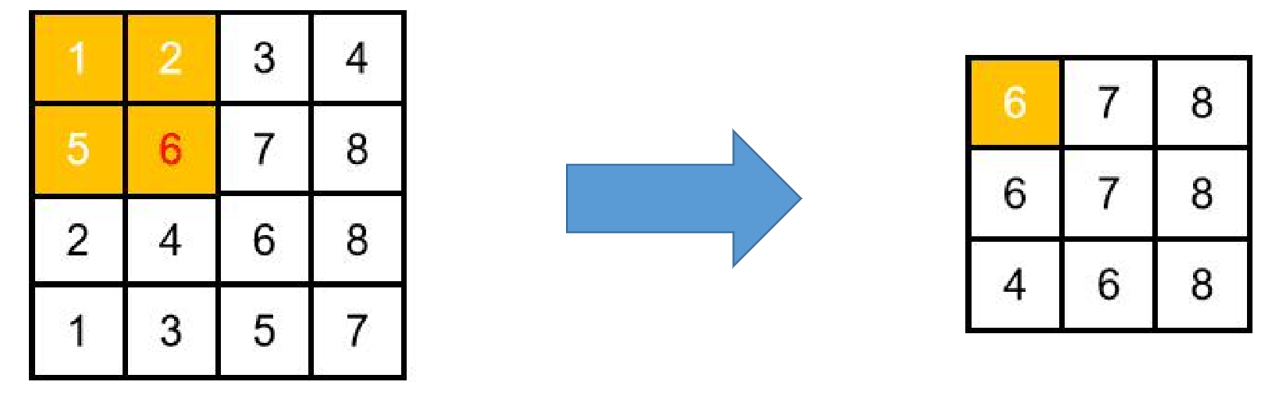
\includegraphics[width = 0.9\textwidth]{maxp.png}
    \caption{最大池化示意图}
    \label{infra}
\end{figure}

图\ref{infra}中展示了整个红外成像的过程,首先经过红外摄像机进行图像采集,由于
红外探测器性能及成本因素,将采集到的模拟信号首先进行模数转换,然后进行
图像处理,最后进行图像的展示或进行目标检测等后续工作。

\subsection{红外图像特性} 
根据红外成像技术原理,结合红外探测器性能的限制以及环境因素,导致红
外图像相比于可见光图像主要有以下特征:

(1)图像分辨率差、对比度低。由于红外图像是吸收红外辐射进行成像的,
而物体的红外辐射在传输过程中经过大气吸收以及环境散射等因素导致红外探
测器接收到的红外辐射会减少,就会导致成像对比度低。

(2)图像信噪比低。红外图像往往会存在着大量的噪声,一部分噪声来自
于设备噪声,由于红外探测器硬件原因会产生热噪声、三粒噪声、光子噪声等。
另一部分来自于环境噪声,这部分因素无法控制。

(3)物体边缘模糊。由于物体之间的热辐射可以相互影响,因此采集到的
图像会出现物体边缘没有明显的界限,这会对后续进行目标检测造成困难。

\section{本章小结}
本章主要介绍了基于深度学习的目标检测算法相关的一些理论基础以及简
要的介绍了红外图像的获取过程。首先对卷积神经网络的组成,包括卷积层、池
化层、全连接层以及激活函数做了详细的介绍,这些都是后续目标检测算法的重
要组成部件。然后介绍了基于深度学习的目标检测算法的性能评价指标以及指标
的计算过程。最后介绍了红外图像相关的知识。简单的概述了红外图像的获取过
程以及红外图像的特性,为后续进行红外图像预处理和网络结构的改进打下理论
基础。
